\chapter{Introduction}
\label{cha:introduction}

Unreachable Code Detection nowadays is integrated in almost every available static code analysis software as well as Integrated Developments Environments and to some extent even compilers.
Unreachable Code is defined as Code that can never be reached, because either the program flow ended prematurely or due to unsatisfiable path conditions.
These types do not only increase the size of the program, but also increase the overall complexity of the sourcecode or may even lead to unwanted behavior and errors (e.g. goto-fail bug) \cite{Boyes_2014}.

\section{Motivation}
Using Static code analysis to find errors before compiling, building or rolling out software is a very essential part of the software development process.
These tools are able to identify a wide range of Errors or make suggestions for adhering to a better style.
Finding errors in sourcecode as it is written will not only make the program more robust, but also makes it more comprehensible, which leads to less time and energy needed during maintenence.
Especially \emph{Unreachable -, Unneccessary - and Dead Code} are a main source of incomprehensible sourcecode \cite{Romano_2020}.
In some instances \emph{Unreachable Code} may be intended due to extensibility of the program \cite{Haas_2020} and may even not be clear if it is intended or not.
Before the break-through of the Object Oriented Paradigm many Programs were developed in an imperative, procedural way. Some Styleguides of that time suggested splitting files into so many smaller Files containing few Functions and/or procedures \cite{Srivastava_1992}.
Interestingly the emerge of the Object Oriented Paradigm and its languages to the de-facto standard increased the precentage of \emph{Unreachable - and Dead Code} \cite{Srivastava_1992}.
In extreme cases Dead Code may even lead to the so called Anti-pattern Lava-Flow \cite{Romano_2020}, which typically occurs when Dead Code will not be removed and has to be maintained, even tough it does not do much or even anything at all.
Systems that undergo constant evolution, like Web Systems, are also prone to Lava-flow and Unreachable Code \cite{Boomsma_2012}.

\section{Technical foundation}
\emph{Unreachable Code} is often confused with similar defects and different definitions are used.
It is often confused with \emph{Dead Code}, but there are also other types besides these two.
\begin{itemize}
  \item \emph{Dead Code} is code that may be reachable, but has no effect on the result. An example of this would be unused variables whose value is the result of a calculation (also known as \emph{Dead Variables}).
  \item \emph{Unreachable Code} is code that will never be, executed because the flow of the program was interrupted.
        This either happens due to statements that interrupt the flow unconditionally (using break, exit, return, goto, et cetera) or conditionally (using if, while, for, et cetera).
  \item \emph{Unnecessary Code} is code that may be deleted. \emph{Unnecessary Code} may still be reachable, but serves no semantic purpose.
\end{itemize}

Analysing these kind if defects requires a representation called \emph{Controlflowgraph} \ref{fig:cfg}, which is a directed graph.
This Graph consists of Blocks, which contain the statements.
Blocks may contain more (or less) than one statement and usually end with either a condition or mark the end of the scope.
Blocks are connected via edges.
These blocks have a maximum of two Edges pointing away, when the last statement contains a condition, since a condition is either true or false.
The first and last block are begin- and endblocks, which contain no statements and their only purpose is to mark the beginning or end of the graph.

% TODO: Description
\begin{figure}
    \begin{GenericCode}
    IF s_operationHour <> m_operationHour THEN
        m_operationHour := s_operationHour;
        IF s_operationHour = 0 THEN
            RESET_ALARM(Name := er_service, SubID1 := m_iNumber);
        END_IF;
        RETURN;
    END_IF;
    // s_operationHour must be equal to m_operationHour
    IF s_operationHour = 0 THEN
        // unnecessary - already zero
        m_operationHour := 0;
        RESET_ALARM(Name := er_service, SubID1 := m_iNumber);
    ELSE
        // unreachable
        IF s_operationHour <> m_operationHour THEN
            s_operationHour := m_operationHour;
        END_IF;
    END_IF;
    \end{GenericCode}
    \caption{A minimal example containing unreachable code due to unsatisfiable conditions. The condition in line 15 is never reachable, since this case was already handeld in line 1 and the state of that variable did not change.}
    \label{code:ex1}
\end{figure}
\begin{figure}
  \centering
  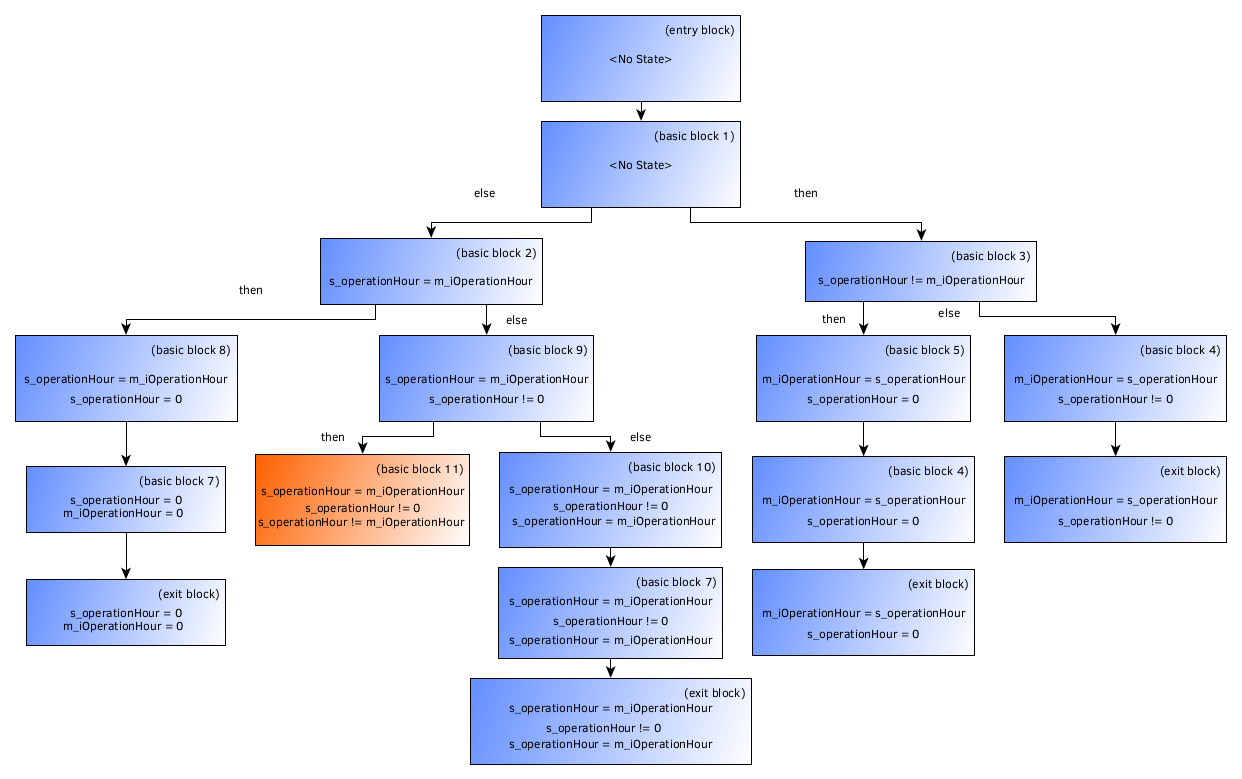
\includegraphics[width=1\textwidth]{minimal-example}
  \caption{The constructed Controlflowgraph of \ref{code:ex1}. Edges are marked either with l - describing the path if the condition results true - or r. Loops (and sometimes gotos) may easily spotted since it is the only possibility for arrows pointing to former nodes.}
  \label{fig:cfg}
\end{figure}

It is worth mentioning that \emph{Controlflow graphs} may be altered to make analysis easier, like \emph {Single static Assignment}, which introduces many artifical variables to prevent redefinition of variables.

\section{Project Overview}
This thesis is written as a part of a research project between the \emph{Software Competence Center Hagenberg GmbH} \cite{ScchGmbH} and \emph{Engel Austria GmbH} \cite{EngelGmbH}.
Engel produces injection molding machines, which are programmed using the \emph{Kemro-IEC} language, a dialect of the \emph{IEC 61131-3} standard language.
The project began as a joint work between the \emph{Software Competence Center Hagenberg} and the \emph{Johannes Kepler University Linz} \mcite{jku}{Prahofer_2012} within the competence centers programme COMET of the Austian Research Promotion Agency (FFG).
Over the years multiple rules identifying a wide range of errors were implemented, for example detecting unguarded division where the divisor could potentially be zero, finding unused variables, highlighting high complexitiy of expressions, detecting Dead Code and other defects.

\section{Objective of this thesis}
Currently a rule for detecting unreachable Code is already in place, but is incomplete.
The only kind of \emph{Unreachable Code} that is detected when Statements stop the \emph{Controlflow} unconditionally (e.g. break, return, exit, goto, etc.).
The goal is to identify as much \emph{Unreachable Code} as possible correctly while minimizing the number of reported false positives.
A popular approch to finding \emph{Unreachable Code} is converting a \emph{Controlflow Graph} into \emph{Single Static Assignment Form} and using \emph{Constant Propagation} \cite{Click_1995}.
Afterwards Condtions may be evaluated if they only consist of constants. The result (either true or false) determines if a given part of sourcecode is always or never will be reachable (as mentioned before, only Conditions with constants only will be evaluated).
This method is efficient and yields good results, but is not able to detect every error.
\begin{figure}
    \begin{GenericCode}
    int $x_0$ $\leftarrow$ 1;
    do { $x_1$ $\leftarrow$ $\phi$($x_0$, $x_3$);
        $b_0$ $\leftarrow$ ($x_{1}$ $\neq$ 1);
        if( $b_0$ )
            $x_2$ $\leftarrow$ 2;
        $x_3$ $\leftarrow$ $\phi$($x_1$, $x_2$);
    } while ( pred() )
    return $x_3$;
    \end{GenericCode}
    \caption{This Problem \cite{Click_1995} is the transformation to Single Static Assignment form, which does not check conditions and inserts a Phi-Function at line 6, even tough the condition in line 4 will never be satisfiable!}
    \label{code:ssa-defect}
\end{figure}
Finding these kind of Errors \ref{code:ssa-defect} requires another approach, which does not rely on the transformation to the Single Static Assignment Form.
Part of this thesis is about using another method for \emph{Unreachable Code Detection}, which is able to find even more instances, while maintaining the same low reporting of false positives.
The developed Method will make usage of a \emph{Satisfiable modulo theory prover} (short: \emph{SMT-Solver}) and \emph{Symbolic Execution} \mcite{Arlt_2013}. The basis of this method will be - again - a \emph{Controlflow Graph}.

At the end the advantages and disadvantages of both algorithms will be discussed and the results will be compared against each other in terms of accuracy and runtime.

% TODO: Fix Inhaltsverzeichnis
% TODO: Seitenzahl eintragen
